\documentclass[11pt]{article}
\usepackage{graphicx} % Required for inserting images
\usepackage[top=2.5cm, bottom=2.5cm, left=2.5cm, right=2.5cm]{geometry}
\usepackage[T1]{fontenc}
\usepackage{hyperref}
\usepackage[utf8]{inputenc}
\usepackage{multirow}
\usepackage{subcaption}
\usepackage{booktabs}
\usepackage{bookmark}
\usepackage{graphicx}
\usepackage{setspace}
\setlength{\parindent}{0in}
\usepackage{physics}
\usepackage{tikz}
\usepackage{tikz-3dplot}
\usepackage[outline]{contour} % glow around text
\usepackage{xcolor}
\usepackage{float}
\usepackage{makeidx}
\usepackage{fancyhdr}
\usepackage{pgfplots}
\usepackage{amsmath}
\pgfplotsset{compat=1.18}
\usepackage{caption}
\usepackage[catalan]{babel}
\setlength{\parskip}{11pt}
\usepackage{xcolor}
\usepackage{listings}
\usepackage{marginnote}
\usepackage{siunitx}
\usepackage{framed}
\usepackage{ulem}


\title{\Huge\bfseries Pràctica 7: \\ Camps magnetics despires i bobines \\ [2ex] \Large}

\author{\begin{tabular}{c}
\textbf{GRUP A6} \\
Isaac Baldi García (1667260)\\
Miguel Ordejón de Prada (1710966) \\
Eira Jacas García (1666616) \\
Víctor Bosch González (1676373)
\end{tabular}}

\date{Abril 2025}

\begin{document}

\maketitle
\begin{center}
    \textbf{Abstract:} 
\end{center}

\newpage
\tableofcontents
\newpage

\section{Introducció}\label{sec: intro}

En aquesta pràctica estudiarem el camp d'inducció magnètica $B$ generat per diferents geometries (espires i bobines). Els objectius que ens plantegem són:

\begin{list}{$\ast$}{\leftmargin=1em}
    \item Comprovar experimentalment la llei de Biot-Savart. Estudiant el camp generat per unes espires al seu centre i les dependències amb el radi i el nombre d'espires. I estudiant el camp generat dins d'una bobina.
    \item Determinar experimentalment la permeabilitat magnètica del buit $\mu_0$.
    \item Comprovar el principi de superposició estudiant diversos sistemes d'espires i bobines amb la mateixa geometria, però amb un major nombre de voltes.
\end{list}

Per tal d'assolir aquests objectius, primer cal saber quina és la llei de Biot-Savart i quins camps resulten d'ella per a espires i bobines.

La llei de Biot-Savart és:
\begin{equation} \label{eq: Biot-Savart}
    \vec{B}(\vec{r}) = \frac{\mu_0}{4\pi}\int_V\frac{\vec{J}(\vec{r'}) \cross (\vec{r}-\vec{r'})}{\abs{\vec{r}-\vec{r'}}^3}d^3r'
\end{equation}

Aplicant-la per obtenir el camp al centre d'una espira i en l'eix d'una bobina, tenim respectivament:
\begin{equation} \label{eq: B_espira}
    \vec{B} = \frac{\mu_0IN}{2R}\hat{z}
\end{equation}
\begin{equation} \label{eq: B_bobina}
    \vec{B} = \frac{\mu_0IN}{2L}\left(\frac{x-L/2}{\sqrt{R^2+(x-L/2)^2}}-\frac{x+L/2}{\sqrt{R^2+(x+L/2)^2}}  \right) \hat{z}
\end{equation}

On $I$ és la intensitat que circula, $N$ és el nombre de voltes que té l'espira o bobina, $R$ és el radi de l'espira o bobina i $L$ és la longitud de la bobina.

\section{Mètode experimental}\label{sec: mètode}

\underline{Muntatge experimental:}
Per dur a terme els experiments, hem muntat el circuit que es mostra en la Fig (\ref{fig: muntatge}). On l'espira o bobina es troba connectada al generador que subministrarà corrent continu i connectada en sèrie a un amperímetre. És important que l'escala de l'amperímetre estigui en 10A i no deixar la intensitat circulant durant massa temps perquè treballarem amb intensitats altes. Alhora, la sonda Hall estarà connectada al teslàmetre i estarà agafada per un suport que permeti moure-la i orientar-la amb facilitat.

Al encendre el teslàmetre, cal esperar a que aquest s'estabilitzi el màxim possible al voltant d'un valor; tot i això, el valor sempre oscil·larà al voltant de $\pm$ 2 mT. Seguidament, ajustar el zero. És possible que durant la realització de l'experiment el teslàmetre es descalibri; en aquest cas, cal tornar a ajustar el zero. Al realitzar mesures amb el teslàmetre, la sonda ha de estar completament alineada amb el camp que es vol mesurar, ja que només mesura la component del camp $B$ paral·lel a aquesta.

A l'hora de fer el muntatge per mesurar el camp de les espires, col·loquem l'espira a un suport mòbil com el de la sonda, de manera que la sonda i l'espira es troben a la mateixa alçada, i la connectem al generador. A l'hora de mesurar el camp d'inducció generat per l'espira, la punta de la sonda s'ha de trobar al centre de l'espira. La punta de la sonda es trobarà just al centre si la distància entre la sonda i qualsevol punt de l'espira és igual al radi de l'espira. Alhora, la sonda estarà alineada amb el camp quan es trobi totalment perpendicular al pla de l'espira. 


El muntatge per mesurar el camp de les bobines consistirà en la regla graduada, la sonda en el suport mòbil i les bobines, elevades per uns blocs de fusta, i connectades al generador. 
Segons la sonda vagi entrant en la bobina, mesurarem la distància recorreguda per saber en quin punt es troba la punta de la sonda relativa al origen. Escollim l'origen just quan la punta de la sonda es troba a l'extrem de la bobina (la part de plàstic); de manera que la posició de la punta de la sonda serà la distància relativa menys la distància des d'on comencen els cables fins on comença la bobina (plàstic).
Per mesurar el camp d'inducció amb la major precisió possible, ens assegurem que la punta de la sonda es troba en l'eix de la bobina a ull (ja que no és possible fer-ho amb el regle com abans); mirant des d'un extrem de la bobina, evitant al màxim possible l'efecte parallax. Com que la sonda ha de entrar sencera dins de la bobina, aquesta ja estarà alineada.



\begin{figure}
    \centering
    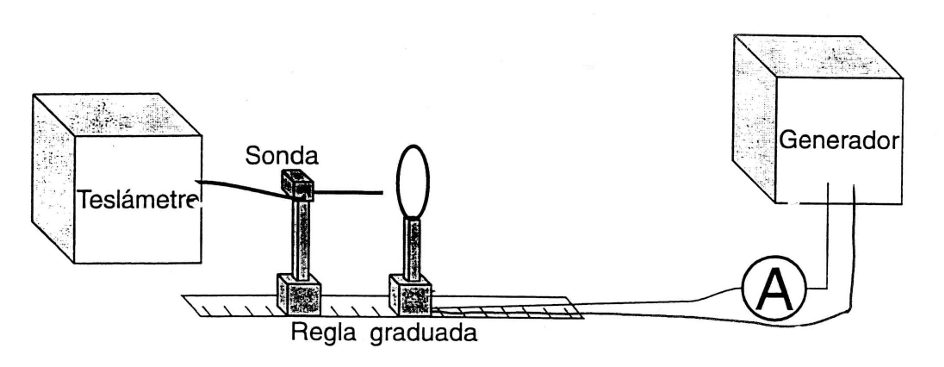
\includegraphics[width=0.75\linewidth]{Muntatge Experimental.png}
    \caption{Muntatge Experimental}
    \label{fig: muntatge}
\end{figure}

Per tal de mesurar únicament el camp generat per les espires o bobines i no cap camp extern. Farem dues mesures del camp però amb la intensitat circulant en sentit oposat. Així, obtenim que el camp generat serà la semidiferència de les dues mesures.
\begin{equation} \label{eq: B_semidif}
    B_{semidif} = \frac{B_+ - B_-}{2}
\end{equation}
D'aquesta manera, qualsevol camp extern que pugui haver-hi (que no variarà en invertir el sentit del corrent), es cancel·larà al fer la resta. És important, pel bon manteniment del generador, cada cop que invertim el corrent; baixar la intensitat a zero,  apagar el generador, canviar els cables i tornar a encendre el generador.

\underline{Obtenció de resultats:} A l'hora d'estudiar el camp generat per una espira (o conjunt d'espires) analitzarem la dependència del camp amb els paràmetres de l'espira mitjançant regressions lineals i el seu coeficient $r^2$. 

La primera dependència que estudiarem serà amb el radi; aquesta, segons la llei de Biot-Savart, ha de ser inversament proporcional. D'aquesta manera, la regressió lineal serà la següent:
\begin{equation}\label{eq: BvsR}
    B=\frac{m}{R} + n
\end{equation}
Per realitzar la regressió, prendrem mesures en tres espires diferents amb radis $R$: $3cm$, $4.25cm$ i $6.75cm$. I amb la resta de paràmetres fixats: $I=1A$ i $N=1$. 

La segona dependència que estudiarem serà amb el nombre de voltes que té el conjunt d'espires; aquesta, pel principi de superposició, ha de ser proporcional. D'aquesta manera, la regressió lineal serà la següent:
\begin{equation}\label{eq: BvsN}
    B=mN + n
\end{equation}
Per realitzar la regressió, prendrem mesures en tres conjunts d'espires amb diferent nombre d'espires $N$: 1, 2 i 3. I amb la resta de paràmetres fixats: $I=1A$ i $R = 6.75 cm$. 

A partir d'aquestes regressions, a més de confirmar la relació entre el camp i el radi i el nombre d'espires, calcularem la permeabilitat magnètica del buit $\mu_0$ comparant les dues rectes de regressió fetes anteriorment i l'expressió teòrica del camp magnètic:

Comparant les Eqs (\ref{eq: B_espira}), (\ref{eq: BvsR}).
\begin{align} \label{eq: mu1}
    m = \frac{\mu_0IN}{2}      \nonumber \\
    \mu_0=\frac{2m}{IN}
\end{align}
I comparant les Eqs (\ref{eq: B_espira}), (\ref{eq: BvsN})
\begin{align} \label{eq: mu2}
    m = \frac{\mu_0I}{2R}        \nonumber \\
    \mu_0=\frac{2Rm}{I}
\end{align}

\section{Resultats experimentals}\label{sec: resultats}
\subsection{Mesaura del camp de les espires}\label{subsec: espires}

En la Fig (\ref{fig:BvsR}) es mostren les dades obtingudes experimentalment del camp d'inducció $B$ enfront de l'invers del radi de les espires $1/R$ (en blau) juntament amb el valor teòric que haurien de tenir (en verd) seguint l'Eq (\ref{eq: B_espira}); es pot observar com les dades experimentals i teòriques són compatibles.
Juntament amb les dades experimentals, la figura presenta una recta de regressió lineal amb un coeficient de correlació \footnote{Les regressions lineals en detall es troben a l'annex \ref{sec: regressions}} $r^2 = 0.9994$ i amb l'equació: 
\begin{equation} \label{reg: BvsR}
    B = (2.7\pm 1.1) \cdot10^{-6} m\cdot T*\frac{1}{R}+(-3 \pm 28)\cdot10^{-6} \, T
\end{equation}
El coeficient de correlació és suficientment elevat com per confirmar una relació lineal entre el camp $B$ i l'invers del radi $1/R$.
Alhora, l'ordenada a l'origen de l'Eq (\ref{reg: BvsR}) és $(-3 \pm 28)\cdot10^{-6}$ T essent compatible amb zero; això ha de ser així per què quan $1/R$ és zero, és a dir $R$ tendeix a infinit, és com si no hi hagués cap espira i, per tant, no ha d'haver-hi cap camp. Per tant, confirmem que el camp és inversament proporcional al radi.

Finalment, a partir de la pendent de la recta de regressió de l'Eq (\ref{reg: BvsR}) i l'Eq (\ref{eq: mu1}) obtenim la $\mu_0$:

\[
\boxed{\mu_0=(1.35\pm0.55)\cdot10^{-6} \, N/A^2}
\]

El resultat de la permeabilitat magnètica del buit $\mu_0$ obtingut a partir de la regressió és compatible amb el valor tabulat de $\mu_0 =$  1.25664 $\cdot 10^{-6}$ N/A$^2$ (REFRERENCIA DEL VALOR).

\begin{figure}[h!]
    \centering
    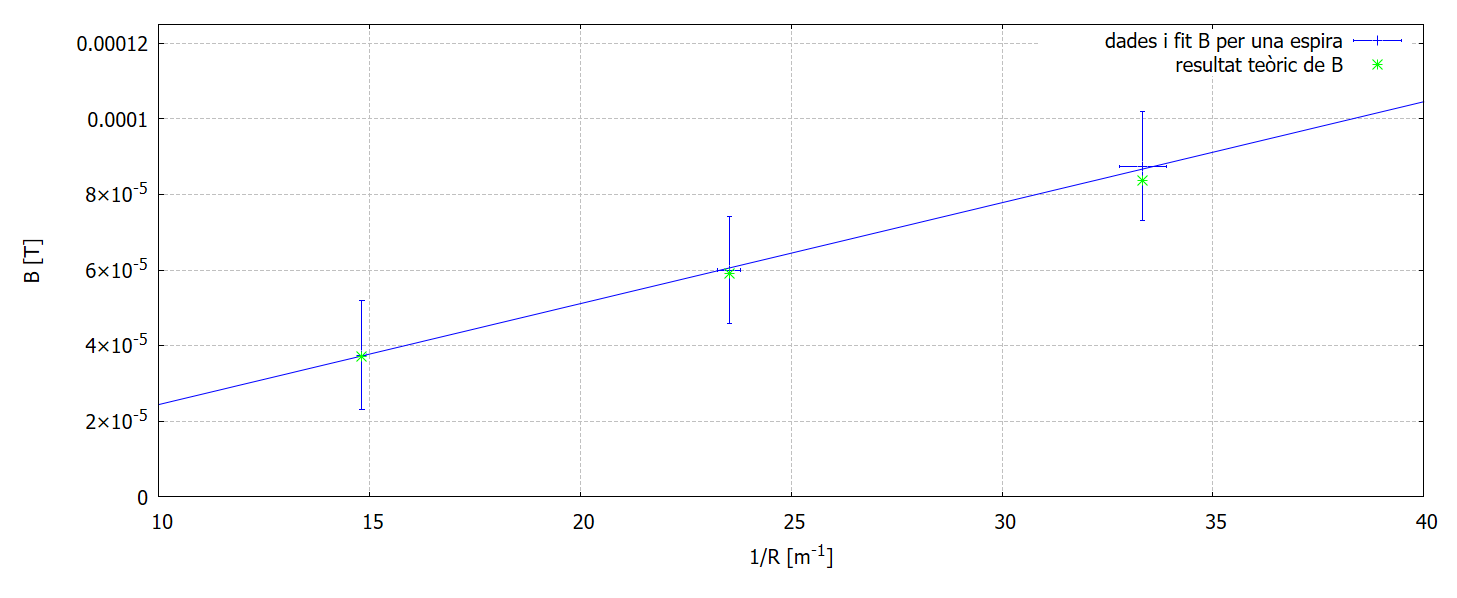
\includegraphics[width=1\linewidth]{BvsR.PNG}
    \caption{Regressió lineal del camp generat $B$ per una espira en el seu centre en funció del invers del seu radi $R$, comparat amb els valors teòrics.}
    \label{fig:BvsR}
\end{figure}

En la Fig (\ref{fig:BvsN}) es mostren les dades obtingudes experimentalment del camp d'inducció $B$ enfront del nombre d'espires $N$ del conjunt (en blau) juntament amb el valor teòric que haurien de tenir (en verd) seguint la fórmula (\ref{eq: B_espira}); es pot observar com les dades experimentals i teòriques són compatibles.
Juntament amb les dades experimentals, la figura presenta una recta de regressió lineal amb un coeficient de correlació de $r^2=0.9987$ i amb una equació:
\begin{equation} \label{reg: BvsN}
    B = [(4.0 \pm 1.0) \cdot10^{-5} *N +(-3 \pm 22)\cdot10^{-6}] \, T
\end{equation}
El coeficient de correlació és suficientment elevat com per confirmar una relació lineal entre el camp $B$ i el nombre d'espires $N$. Alhora, l'ordenada a l'origen de la recta (\ref{reg: BvsN}) és $(-3 \pm 22)\cdot10^{-6} \, T$ essent compatible amb zero i el pendent d'aquesta és $(4.0 \pm 1.0)\cdot10^{-5}$ T compatible amb el valor del camp d'inducció $B$ per a una única espira $3.723\cdot10^{-5}$ T; això ha de ser així pel principi de superposició: fent que els camps de les espires individuals es sumin; però, com que són espires iguals i es troben prou a prop, el camp total és el nombre d'espires multiplicat pel camp que genera una única espira, i quan no hi ha espires el camp ha de ser zero. Per tant, confirmem que el camp és proporcional al nombre d'espires.

Finalment, a partir de la pendent de la recta de regressió de l'Eq (\ref{reg: BvsN}) i l'Eq (\ref{eq: mu2}) obtenim la $\mu_0$:

\[
\boxed{\mu_0=(1.35\pm0.34)\cdot10^{-6} \, N/A^2}
\]

El resultat de la permeabilitat magnètica del buit $\mu_0$ obtingut a partir de la regressió és compatible amb el valor tabulat de $\mu_0 = 1.25664\cdot 10^{-6} N/A^2$.

\begin{figure}[h!]
    \centering
    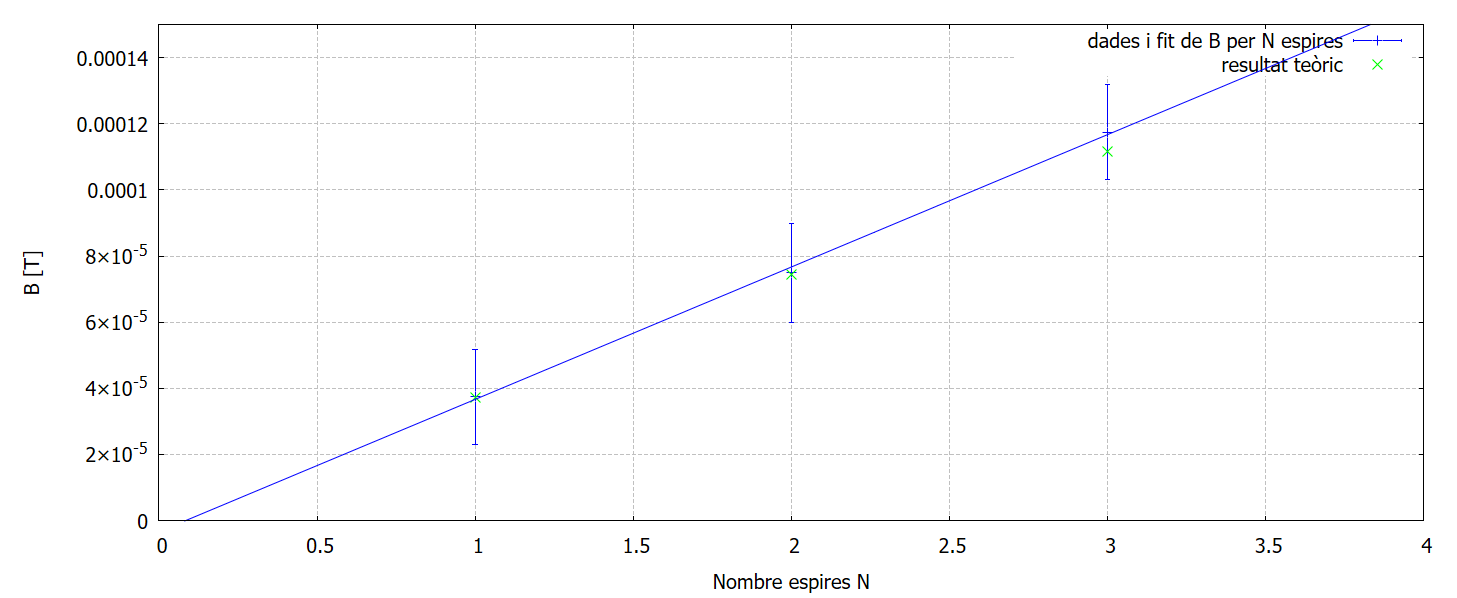
\includegraphics[width=1\linewidth]{BvsN.PNG}
    \caption{Regressió lineal del camp generat $B$ per a un conjunt de $N$ espires en funció del nombre d'espires $N$, comparat amb els valors teòrics.}
    \label{fig:BvsN}
\end{figure}

Mitjançant tots dos mètodes obtenim un valor de la permeabilitat $\mu_0$ que és compatible amb el valor tabulat. Per tant, tots dos mètodes són vàlids per trobar la permeabilitat. Però, donat que la incertesa del segon mètode és menor, considerem que aquest és millor per mesurar la permeabilitat $\mu_0$.


\subsection{Mesura del camp de les bobines}\label{subsec: bobines}

\begin{figure}[h]
    \centering
    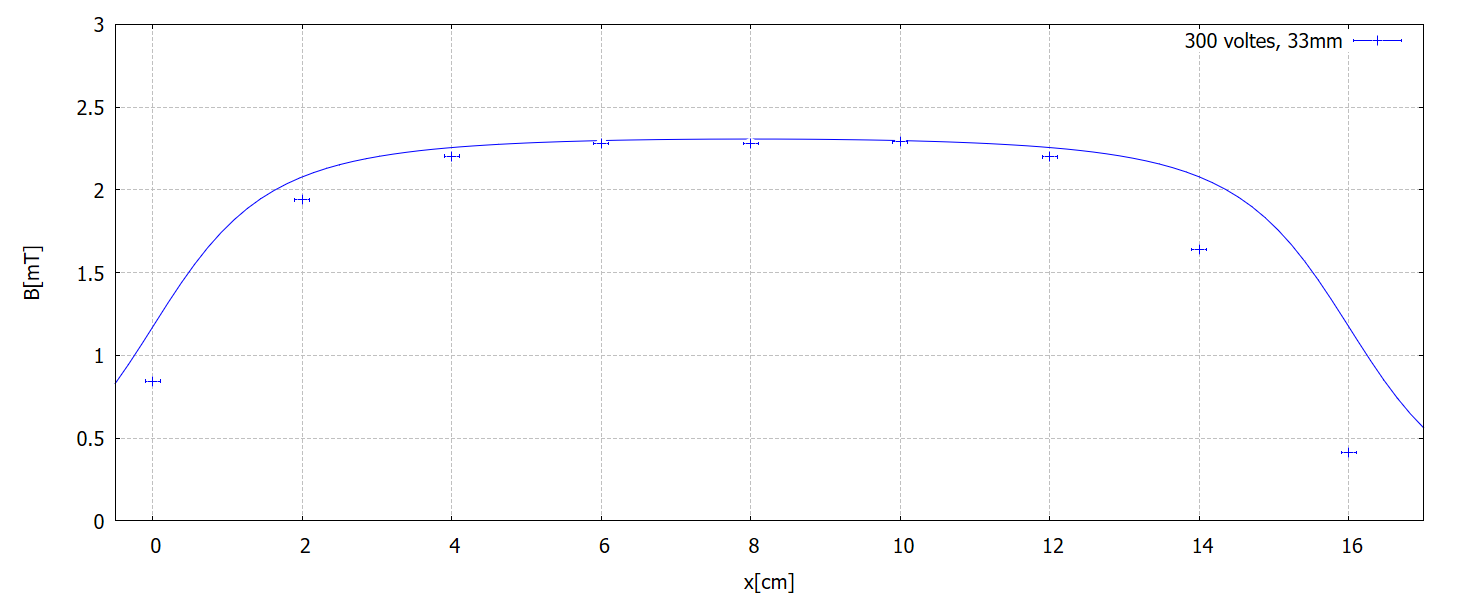
\includegraphics[width=0.75\linewidth]{Bobina 1.PNG}
    \caption{Camp d'inducció $B$ en l'eix d'una bobina (33mm de diàmetre, 16 cm de longitud i 300 voltes) en funció de la posició $x$. Punts experimentals i valor teòric.}
    \label{fig: BvsX_33mm}
\end{figure}

En la Fig (\ref{fig: BvsX_33mm}) podem veure com el camp d'inducció mesurat proper al centre de la bobina (2.285 $\pm$ 0.014)mT és compatible amb el camp teòric 2.298 mT. Però, els valors mesurats en els extrems de la bobina són significativament més baixos que els valors teòrics. Això pot ser degut a què no vàrem mesurar exactament a l'eix de la bobina: on en el centre té, aproximadament, el mateix valor, però cap als extrems el camp decau més ràpidament. (REFERENCIAR LA INFO O FER NOSALTRES LA SIMULACIÓ)

Aquest error es deu a que el nostre mètode per saber si la sonda es troba a l'eix (descrit a la secció \ref{sec: mètode}) és poc exacte. Un mètode més exacte seria mesurar amb el regle la distància entre la part de la sonda que està fora de la bobina i l'exterior de la bobina i, si aquesta es troba a un radi de distància, la part de la sonda mesurada es trobarà en l'eix. I, com que la sonda ha d'estar alineada amb el camp d'inducció, tota la sonda es trobarà en l'eix.

\begin{figure}[h]
    \centering
    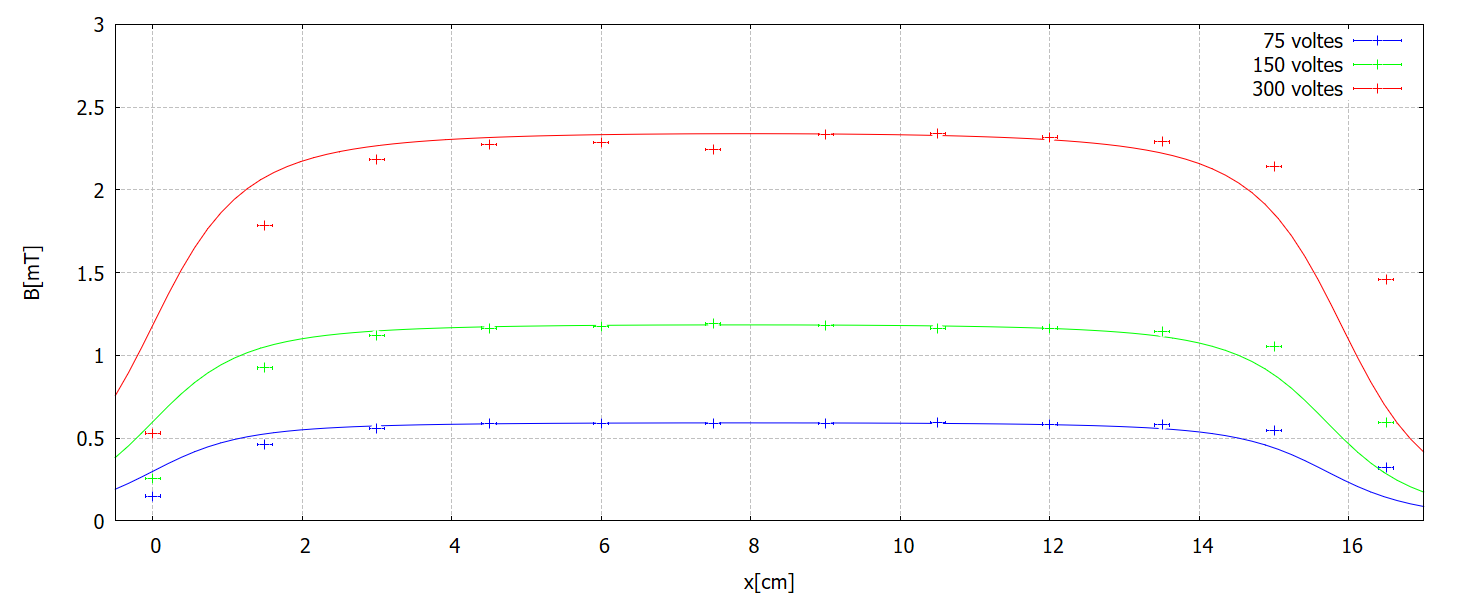
\includegraphics[width=0.75\linewidth]{Bobines 2,3,4.PNG}
    \caption{Camp d'inducció $B$ en l'eix de tres bobines diferents (26mm de diàmetre i 15.8 cm de longitud) en funció de la posició $x$. Punts experimentals i valor teòric.}
    \label{fig: BvsX_26mm}
\end{figure}

En la Fig (\ref{fig: BvsX_26mm}) podem veure com el camp d'inducció mesurat al voltant dels 6 a 12 cm de les bobines és de (0.590 $\pm$ 0.014)mT, (1.180 $\pm$ 0.014)mT i (2.335 $\pm$ 0.014)mT, és compatible amb el camp teòric 0.591 mT, 1.184 mT i 2.338 mT, respectivament. Però a l'inici, el valor mesurat és significativament menor i al final, significativament més gran. Aquesta desviació respecte del valor teòric pot ser deguda a què no vàrem començar a mesurar en l'origen.

Per tal de comprovar aquesta hipòtesi, hem realitzat el mètode dels mínims quadrats \footnote{El mètode dels mínims quadrats es troba explicat a l'annex \ref{sec: mínims_quadrats}} per trobar si hi ha un origen on tots els punts experimentals són compatibles. Al aplicar-ho, trobem que per a les tres bobines el nostre origen es trobava 8 mm desplaçat cap a fora. En la Fig (\ref{fig: Bvsx_26mm}), on es mostren les dades experimentals i teòriques tenint en compte aquest desplaçament de 8 mm, es veu que totes les dades experimentals de les tres bobines són compatibles amb els valors teòrics, excepte el punt a 7.5 cm de la bobina de 300 voltes, que és considerablement menor.

\begin{figure}[h!]
    \centering
    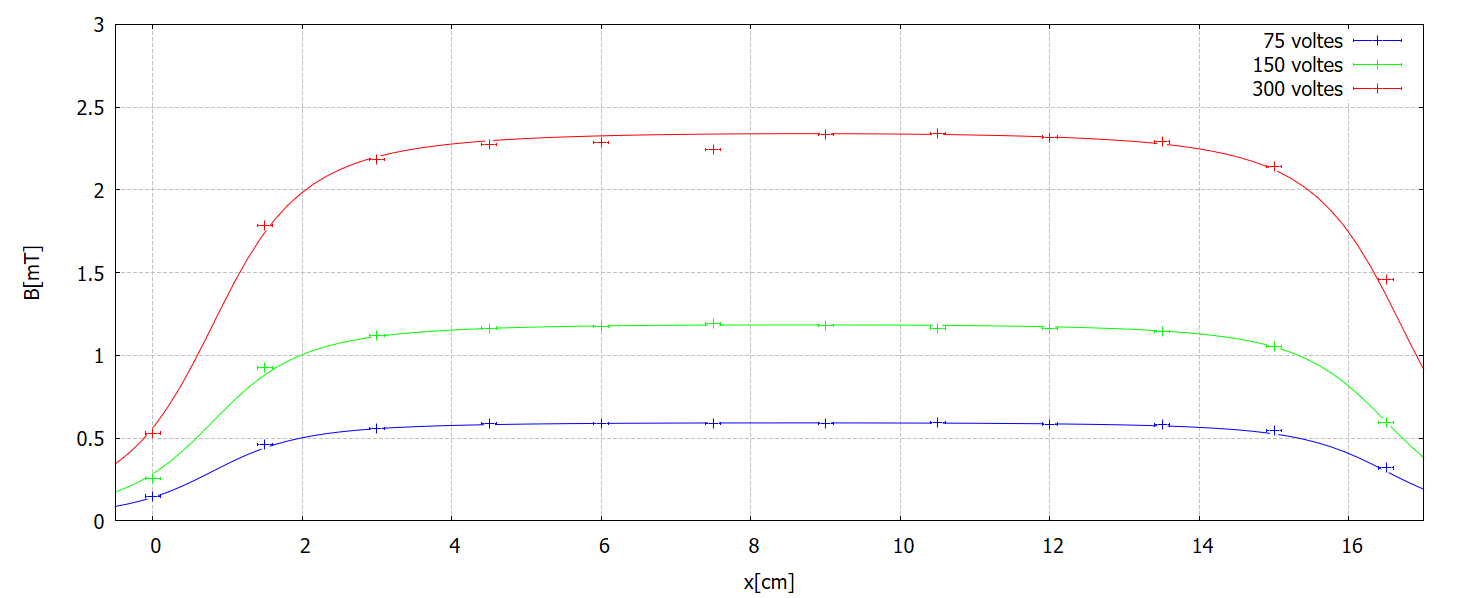
\includegraphics[width=0.75\linewidth]{Bobines 2,3,4 shift 8mm.PNG}
    \caption{Camp d'inducció $B$ en l'eix de tres bobines diferents (26mm de diàmetre i 15.8 cm de longitud) en funció de la posició $x$. Punts experimentals i valor teòric amb l'origen desplaçat.}
    \label{fig: Bvsx_26mm}
\end{figure}

Donat que amb el desplaçament de 8 mm del origen tots els punts, excepte un, són compatibles, confirmem que aquest és el motiu de la desviació entre l'experiment i la teoria. Aquest error es deu a que el nostre mètode per trobar l'origen de la bobina (descrit a la secció \ref{sec: mètode}) és poc exacte. Un mètode més exacte és usar bobines d'un plàstic transparent, de manera que l'origen seria el punt on la punta de la sonda es troba just entrant en els cables; les demés posicions se seguirien trobant amb el mètode de la distància relativa, ja que els cables seguirien essent opacs. Un altre mètode més exacte és posar un petit sensor de proximitat a la punta de la sonda i tapar un dels extrems de la bobina; de manera que el sensor mesura la distància de la punta a la tapa i la posició de la punta és aquesta distància menys la distància de la tapa al inici dels cables.

D'altra banda, comparant el valor del camp entre elles (bobines de dimensions iguals i diferent nombre de voltes), fent el quocient entre els camps per a cada bobina en cada punt, trobem que el camp per 300 voltes és aproximadament el doble que el de 150 i aquest, alhora, és aproximadament el doble que el de 75 \footnote{Els valors del camp i els quocients es troben a l'annex \ref{sec: dades_experimentals}}. Pel que veiem, el camp generat per una bobina és proporcional al nombre de voltes. Confirmant el principi de superposició.


\section{Conclusions}\label{sec: conclusions}
En aquesta pràctica hem estudiat el camp d'inducció magnètica generat per espires i bobines de diferents radis i nombre de voltes. 

En primer lloc, hem estudiat les dependències amb el radi i el nombre de voltes del camp d'inducció generat per una espira en el seu centre. Obtenint que el camp és proporcional al nombre de voltes i inversament proporcional al radi de l'espira. Concordant amb el resultat teòric obtingut a partir de la llei de Biot-Savart. A més, comparant les dependències obtingudes amb la fórmula experimental hem obtingut dos valors de la permeabilitat magnètica del buit $\mu_0$ = (1.35 $\pm$ 0.55)$\cdot10^{-6}$ N/A$^2$ i $\mu_0$ = (1.35 $\pm$ 0.34)$\cdot10^{-6}$ N/A$^2$, tots dos compatibles amb el valor tabulat de $\mu_0 =$  1.25664 $\cdot 10^{-6}$ N/A$^2$.

En segon lloc, hem estudiat el camp generat per diferents bobines al llarg del seu eix. Obtenint perfils del camp d'inducció que en el centre són compatibles amb el resultat teòric, però que en els extrems no ho són. Deduïm que aquests errors es deuen a una metodologia inexacta. A més, comparant els perfils obtinguts per tres bobines de la mateixa geometria però amb diferent nombre de voltes, observem que els camps d'inducció són proporcionals al nombre de voltes; resultat compatible amb el principi de superposició.

\newpage
\appendix{Annex}
\section{Càlcul d'incerteses}\label{sec: incerteses}
\underline{Incertesa estadística d'un conjunt de mesures:}
Com a incertesa de qualsevol longitud mesurada hem agafat $u_d = 10^{-3}m$, que és la distància mínima que les regles podien mesurar.
Per les incerteses de les intensitats i camps d'inducció no hem agafat el valor mínim que podien mesurar l'amperímetre i teslametre perquè tots dos no donaven un valor fix; hem agafat el rang de valors on oscil·lava la mesura $u_I = 10^{-3}A$ i $u_B = 2 \cdot 10^{-5}T$.

\underline{Incertesa estadística de la mitja d'un conjunt de mesures:} La fórmula per trobar l'incertesa estadística d'un conjunt de mesures és:
\begin{equation} \label{eq: incertesa estadística}
    u^2 = \frac{1}{N(N-1)} \sum_{i=1}^{N} (x_i - <x>)^2
\end{equation}
on ${x_i}$ són les variables mesurades, $<x>$ la seva mitjana i $N$ el nombre de variables mesurades.

\underline{Incertesa total:} Per obtenir l'incertesa total d'una mesura a partir de les incerteses estadístiques i instrumentals usem:
\begin{equation} \label{eq: incertesa total}
    u_{Total}^2 = u_{ins}^2+u_{est}^2
\end{equation}

\underline{Propagació d'errors:}  Per trobar les incerteses de magnituds dependents d'altres magnituds mesurables hem usat l'equació de propagació d'incerteses
\begin{equation} \label{eq: propagació d'errors}
    u_{y}^2=\sum_{i=1}^{N}(\frac{\partial y}{\partial x_i})^2u_{x_i}^2
\end{equation}
on y és la magnitud dependent i ${x_i}$ les variables mesurables.

L'incertesa de l'Eq (\ref{eq: B_semidif}) :
\begin{equation}
    u_{B_{semidif}} = \frac{u_{B,ins}}{\sqrt{2}}
\end{equation}

L'incertesa del invers de qualsevol magnitud x:
\begin{equation}
    u_{\frac{1}{x}} = \frac{u_x}{x^2}
\end{equation}

L'incertesa de $\mu_0$ de l'equació (\ref{eq: mu1}):
\begin{equation}
    u_{\mu_0}^2 = \left(\frac{2}{IN}\right)^2u_m^2 + \left(\frac{2m}{I^2N}\right)^2u_I^2
\end{equation}

L'incertesa de $\mu_0$ de l'equació (\ref{eq: mu2}):
\begin{equation}
    u_{\mu_0}^2 = \left(\frac{2R}{I}\right)^2u_m^2 + \left(\frac{2m}{I}\right)^2u_R^2 + \left(\frac{2Rm}{I^2}\right)^2u_I^2
\end{equation}

\section{Regressions lineals} \label{sec: regressions}

 Per fer regressions lineals que tenen en compte les incerteces individuals de cadascun dels punts, hem utilitzat el mètode de mínims quadrats ponderats (weighted least squares).
 
 Donada una funció $f(x,\vec{\beta})$ a ajustar (en el nostre cas $f(x) = mx+n$):
 \begin{equation}
     f(x,\vec{\beta}) = \sum_{j=1}^m\beta_j\phi_j(x)
 \end{equation}
 
  On ${\beta_j}$ són els paràmetres a ajustar i $\phi_j$ són funcions de x (en el nostre cas $\phi_1 = x$, $\beta_1 = m$ i $\phi_2 = 1$, $\beta_2 = n$)
 
 \begin{equation}
     \hat{\beta} = (X^TWX)^{-1}X^TW\vec{y}
 \end{equation}
 \begin{equation}
     M^\beta = (X^TWX)^{-1}
 \end{equation}
 
 On $\hat{\beta}$ és l'estimador de $\beta$, $M^\beta$ la matriu de variància dels estimadors, d'on els elements de la diagonal són la desviació estàndard al quadrat dels estimadors i, per tant, l'incertesa és l'arrel quadrada dels elements de la diagonal. $W$ és la matriu (diagonal) de ponderació, $X$ és la matriu de les variables independents i $\vec{y}$ el vector de la variable dependent.
 
 \begin{equation}
     W_{ii} = \frac{1}{\sigma_i^2}
 \end{equation}
 \begin{equation}
     X_{ij} = \phi_j(x_i)
 \end{equation}

Obtenim el coeficient de determinació $R^2$ mitjançant la fórmula:
\begin{equation}
    R^2 = 1 - \frac{SS_{res}^\omega}{SS_{tot}^\omega}
\end{equation}
\begin{equation}
    SS_{tot}^\omega = \sum^n_{i}(\omega_i(y_i-\overline{y}))^2
\end{equation}
\begin{equation}
    SS_{res}^\omega = \sum^n_{i}(\omega_i(y_i-\hat{y}_i))^2
\end{equation}
on $\overline{y}$ és la mitjana dels valors de $y$ i $\hat{y}$ és el valor predit per l'estimació.

\section{Mètode dels mínims quadrats} \label{sec: mínims_quadrats}

El mètode dels mínims quadrats es basa en optimitzar els paràmetres $\lambda_i$ d'una funció $f(x;\lambda_1,...,\lambda_n)$ de tal manera que l'error quadràtic $\epsilon^2$ entre el valor experimental $y(x)$ i el predit per la funció $f(x)$ sigui el mínim.
\begin{equation}
    \epsilon^2 = \sum_j(y_j-f_j)^2
\end{equation}
És a dir, quan les derivades parcials de l'error respecte als paràmetres siguin zero.
\begin{align}
     & \frac{\partial}{\partial\lambda_i}\epsilon^2 = 0 \, , \,\,\,\, \forall \lambda_i
\end{align}
    
\section{Dades experimentals} \label{sec: dades_experimentals}

\begin{tabular}{|c|c|c|c|c|c|}
            \hline
            x(cm)	&	B$_{75}(mT)$   & B$_{150}$ (mT)    & B$_{300}$ (mT) &	 B$_{150}$/B$_{75}$ & B$_{300}$/B$_{150}$ \\\hline
            0.0 ± 0.1 	&	0.150 ± 0.014   & 0.255 ± 0.014     & 0.530 ± 0.014     & 1.7  & 2.1
	\\\hline
            1.5 ± 0.1	&	0.460 ± 0.014   & 0.925 ± 0.014     & 1.785 ± 0.014     & 2.0  & 1.9
	\\\hline
            3.0 ± 0.1	&	0.560 ± 0.014   & 1.120 ± 0.014     & 2.185 ± 0.014     & 2.0  & 2.0
	\\\hline
            4.5 ± 0.1	&	0.590 ± 0.014   & 1.165 ± 0.014     & 2.275 ± 0.014     & 2.0  & 2.0
	\\\hline
            6.0 ± 0.1	&	0.590 ± 0.014   & 1.175 ± 0.014     & 2.285 ± 0.014     & 2.0  & 1.9
	\\\hline
            7.5 ± 0.1	&	0.590 ± 0.014   & 1.190 ± 0.014     & 2.245 ± 0.014     & 2.0  & 1.9
	\\\hline
            9.0 ± 0.1	&	0.590 ± 0.014   & 1.180 ± 0.014     & 2.335 ± 0.014     & 2.0  & 2.0
	\\\hline
            10.5 ± 0.1	&	0.595 ± 0.014   & 1.165 ± 0.014     & 2.340 ± 0.014     & 2.0  & 2.0
	\\\hline
            12.0 ± 0.1  &   0.585 ± 0.014   & 1.165 ± 0.014     & 2.320 ± 0.014     & 2.0  & 2.0
        \\\hline
            13.5 ± 0.1  &   0.580 ± 0.014   & 1.145 ± 0.014     & 2.290 ± 0.014     & 2.0  & 2.0
        \\\hline
            15.0 ± 0.1  &   0.545 ± 0.014   & 1.055 ± 0.014     & 2.140 ± 0.014     & 1.9  & 2.0
        \\\hline
            16.5 ± 0.1  &   0.320 ± 0.014   & 0.595 ± 0.014     & 1.460 ± 0.014     & 1.9  & 2.5
        \\\hline
\end{tabular}

\end{document}
